\fancyhead[LO]{{\scriptsize {\FA \ }我们最幸福 {\FA } 人人自危}}%奇數頁眉的左邊
\fancyhead[RO]{{\tiny{\textcolor{Gray}{\FA \ }}}\thepage}
\fancyhead[LE]{{\tiny{\textcolor{Gray}{\FA \ }}}\thepage}
\fancyhead[RE]{{\scriptsize {\FA \ }我们最幸福 {\FA } 人人自危}}%偶數頁眉的右邊
\fancyfoot[LE,RO]{}
\fancyfoot[LO,CE]{}
\fancyfoot[CO,RE]{}
\chapter*{12 {\FA } 人人自危}
\addcontentsline{toc}{chapter}{\hspace{5mm}12 {\FA } 人人自危}
\begin{figure}[!htbp]
	\centering
	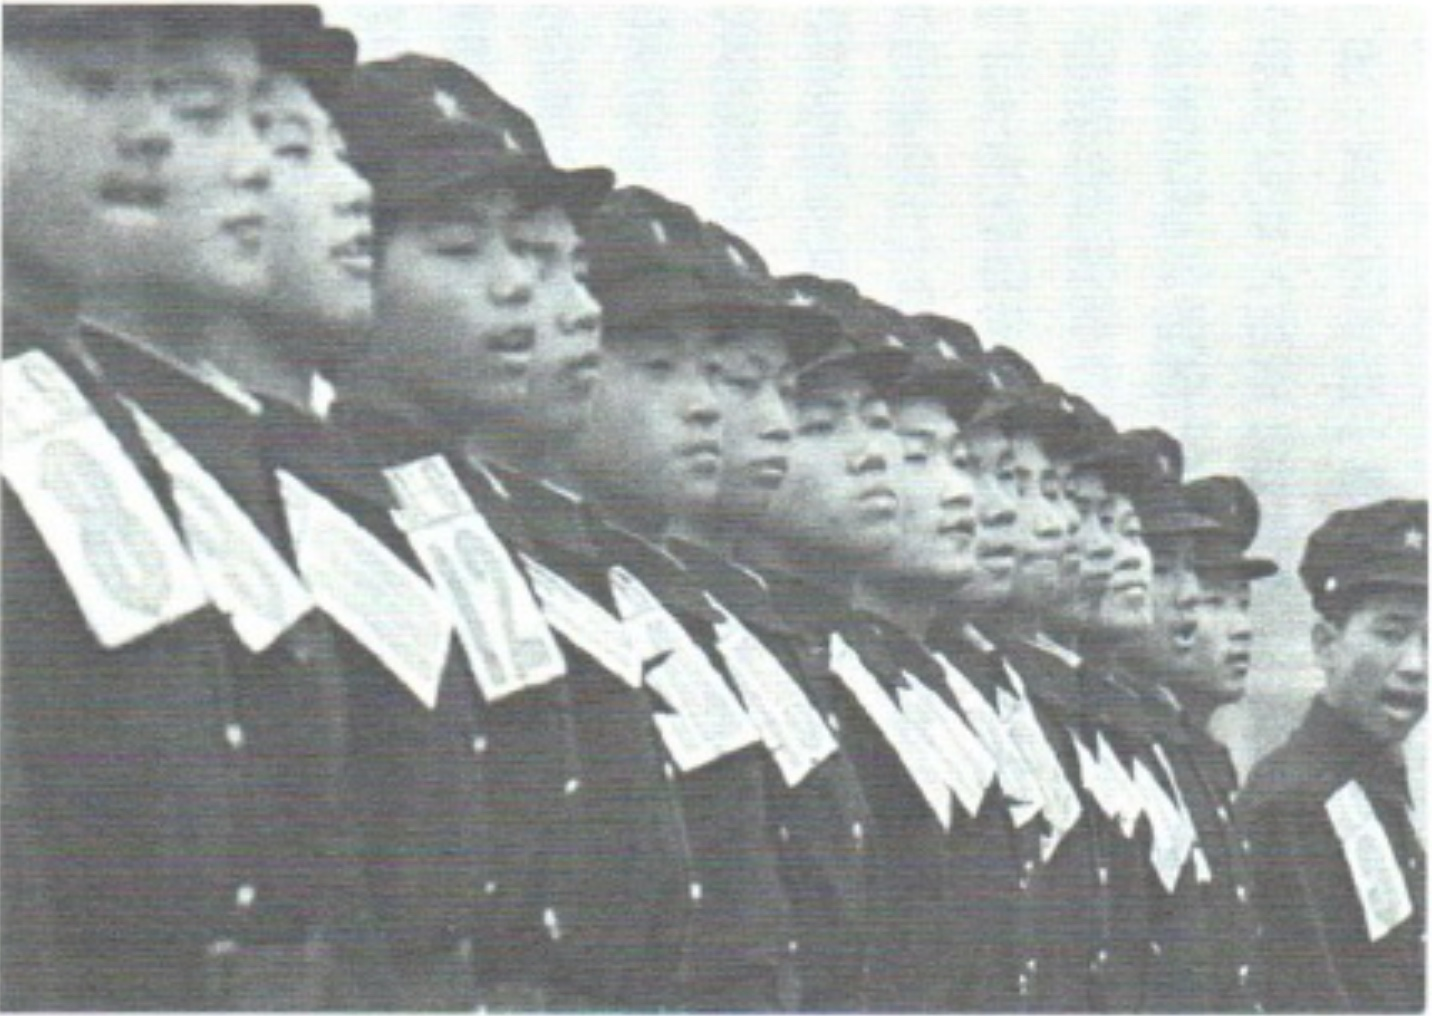
\includegraphics[width=6cm]{./Chapters/Images/12.jpg}
	\caption*{平壤北朝鲜警卫立正列队}
\end{figure}


正如因纽特人有着丰富的词汇描述冰雪,北朝鲜人有着大量的字眼形容罪犯。一些人仅仅是因为微小的过错──例如翘班──就会被送去拘留所(Jibkyulso)\footnote{拘留所是由基层警察单位──人民安全署运作的拘留中心。}或者被关进Rodong Danryeondae劳动锻炼队\footnote{劳动营在哪里会被判处1-2个月的重体力劳动,例如铺路。}。\\

最臭名昭著的监狱是管理所(Kwanliso)──字面意义是”控制及管理所。”事实上,就是劳动营殖民地,在这个国家最北的大山里,延绵数公里。卫星图像显示,这里大约关押这20万人。仿造苏联的古拉格\footnote{古拉格是苏联时期的劳动营。──译者},金日成刚刚掌权就建造了这个集中营,将任何对他有威胁的人投入这里,包括政治上的竞争者,地主或通敌日本的朝奸后代,基督教传教士。在那里,有的人因阅读外国报纸,有的人因酒后拿金正日的身高开玩笑而被抓。“侮辱当局领导人”是被称为“颠覆国家”的最严重的罪行。宋女士工厂的一个女工,因为在日记里写了些政治上不正确的东西而被带走。我认识的北朝鲜人,他们常常会私下里议论,他们认识的或者听说的人,突然半夜里消失了后就再也没有回来。一旦被送进管理所,就是终身监禁。孩子,父母或者兄弟姐妹通常会被一起带走,以铲除三代以内的所谓“不洁之血”。由于不是血亲,配偶通常会被放过,被强制离婚。管理所之内到底会发生些什么,没人知晓,几乎没人能活着逃出那里,讲述他们的遭遇。\\

另外一种类型的劳动营称为教化所(Kyohwaso),字面意思是“管教中心。”反映设立这个机构的初衷是改造那些叛逆、顽劣之徒。这是针对那些非政治犯罪,例如非法越境,走私,或者仅仅是做私人买卖的人而设立的。这些劳动营不如那些关押政治犯罪的劳动营那么可怕,因为理论上说,这些罪犯可以刑满释放──前提是他或她能想方设法活下来。\\

金赫在16岁生日过后不久就被捕了。当时,他待在稳城一个朋友的家里,朋友家离孤儿院不远,是他认识的人里面家离孤儿院最近的,也是一旦他累的不行之后的去处。当时他刚刚从中国返回──由于频繁的往来中国,结果就是,他被警方盯上了。\\

当时,金赫在等着8月里白天的热浪消下去,这样他可以出去砍些柴。大概下午4点的时候,他从屋子走到后院。他看见一个人,然后又有一个,看着自己。他看到他们,就注意到这些人虽然都没有穿制服,但是他们的目光让他强烈的感觉到,这些人是来找自己的。他拿起斧子,慢慢的转到房子前面,想着翻过院墙赶紧跑。但是在房前他看到更多的人。可能一共有8个。所以他只好站住,镇定的开始劈柴,期待用劈柴时木片的四处飞溅来驱赶自己内心的恐惧,稳定下自己狂跳的心脏。\\

便衣警察把金赫押到了稳城郡市中心一栋楼里的一间办公室。他们来自保卫部(Bowibu),调查政治犯罪的国家安全局。事情比他想象的要严重的多。在中国的时候,金赫曾经给几个想潜入北朝鲜的中国商人画了一张地图。在北朝鲜这几乎等于叛国,按北朝鲜刑法五十二条,叛国罪的规定:“任何共和国公民,潜入外国或敌国,包括在外国大使馆寻去庇护……(或)协助敌对国家公民及机构,提供诸如向导,通译的服务或提供道义、物质上的帮助……应被判处死刑。”\\

在一根方形木棒的帮助下,金赫很快就招供了。他们用木棒打金赫的背、肩膀、腿和脚板,实际上,为了让他保持意识,除了头,他们哪里都打。他把自己蜷成婴儿状以避开击打。在那里,警察没有拘留所,只有办公室。所以他们把他铐在一个非常小的房间里,房间小的他无法躺下来,以至于他想将遍体鳞伤的身体靠一靠墙都痛苦万分。晚上他无法入睡,然而到了白天,即使在挨打的时候,他又昏昏欲睡,或者丧失知觉。金赫不知道还能期待什么。虽然历经坎坷,他以前只被抓过一次──就是十岁的时候偷糯米饼的那次。他是那种总是能够虎口脱险的孩子。现在,情况不同了,他被当成一个成人,犯有严重罪行的罪犯。他感到无助、失败、没有尊严。在审讯期间,他絮絮叨叨。他告诉审讯人员任何他们想知道的事情,但他们只想知道中国商人在哪里,而这是金赫真的不知道的。\\

几个月后,他们把他转移到普通的县监狱,在那里他又遭到新一轮的殴打。\\

金赫没有接受审判,但是国家安全警察最终放弃了对他叛国罪的指控,因为他们找不到中国商人,也不想让案子悬着。金赫最后被控以非法越境。这本身就是很严重的罪行了,判处入劳动营3年。\\

第十二教化所坐落于另外一个边境城市──会宁市,在稳城郡以南65公里。金赫被手铐铐着乘火车到了那里。在火车站,他遇到了解送至此的其它几个罪犯。用绳子系成一串,他们列队从城里走向山里的劳动营营地。当他们到达的时候,引擎轰鸣,带动厚重的铁门吱吱呀呀,徐徐的打开。大门的顶上是金日成的语录。金赫对这里心生畏惧,以至于不敢抬眼看看这些标语。\\

金赫先被送去医疗室,在哪里他被测了身高、体重。劳动营没有制服,犯人们都穿着自己的衣服。如果衣服有领子,他们就会把领子剪掉,因为在里面领子是地位的象征,被劳教的服刑人员是没有资格穿的。任何颜色鲜艳的衣服都会被拿走。金赫在中国买的蓝夹克就被狱警没收。另外一个囚犯拿走了他的运动鞋。\\

具金赫估计,这个劳动营里大概关押有1500人,大多数都是年长男性。金赫是那时年纪最小的,但不是最弱的。金赫很吃惊在国家安全特工手里,他吃的很好──由于他们手上只有几个罪犯,因此警察们去市场上买来面条给囚犯吃。在监狱吃了第一顿之后,金赫马上就明白了为什么那些大叔看上去一个个皮打皱,瘦的不成人形,为什么他们的肩膀突在衬衣下面,像个衣服架子。一个警卫给他了一个叫米团子的东西,其实里面大多数是玉米、玉米棒、玉米壳和叶子。比网球大不了多少,金赫很容易一手就包了起来。这就是正餐。有些时候,除了米团子,他们会有些豌豆吃。\\

囚犯们早上7点就要出工,开始劳动一直到日落。劳动营其实就是个繁忙的大工厂,有木料场、砖厂、煤矿和一个农场。劳动营制造从家具到自行车的所有产品。金赫被分配到伐木组。因为他很矮,因此他负责记录其它人砍伐的木头数量。他还要负责登记犯人的休息时间。金赫并不认为做这个很幸运。他怎么可能对那些早他进来十几年的老犯人进行管理呢?\\

“对他们的任何惩罚,你也有份。”给金赫分工的警卫这样向他咆哮。“如果他们任何人试图逃跑,他们会被枪毙,你也会。”\\

虽然金赫没有看见,但是确实有人想逃跑。那个人偷偷溜出他的工作小组,穿过树林,找着逃跑的路。但是劳动营的围墙有3米高,顶上满是带锋利尖角的铁丝网。那个人整夜都在树林里跑来跑去,最后还是回来,跪在监狱大门口祈求宽恕。实际上,他们绕了他的命,声称这是“慈爱领袖的宽宏大量”\\

囚犯们除了在吃饭、睡觉和意识形态学习时之外,不允许停止劳作。在新年假日里,他们要反复诵读金正日的新年致辞,直到逐字逐句的背下来。“今年,我们的人民应该加快前进速度,坚定拥护我们在思想,军队,科学和技术等各个领域的重要方针。”\\

到了晚上,囚犯就直接睡在水泥地板上,每个房间50人。因为只有寥寥数床毯子,人们只好挤在一起相互取暖。有时候一床毯子下能睡10个人。到了晚上,人们筋疲力尽,没人聊天,一个个背靠背或者相互抱着别人的脚就睡着了。为了让一床毯子多盖几个人,他们都是头、脚间隔着睡,按这样的方式每个人都把自己的臭脚给了别人。\\

刚到的时候,金赫像害怕警卫一样害怕其它的囚犯。他以为那些人都是十恶不赦的犯罪分子,都是些可怕的,暴力的人,都是性侵害罪犯。实际上,饥饿的另外一个好处就是使人们丧失了性欲。在劳动营里,几乎没有性行为,连打架都很少。除了那个拿他鞋的人,其它囚犯的暴力程度大多都不如他在火车站流浪时所遇见的孩子。他们大多数都是“经济罪犯”,都是在边境或者市场上惹了麻烦。他们之中的盗窃犯也就是偷了些吃的而已。他们中有一个40岁左右的农夫,原来在集体农庄里养牛。他的罪行就是没有向上报告刚出生就死去的小牛犊,而是把死牛犊带回家,给妻子、和两个年幼的孩子吃了。在金赫遇到这个人的时候,他10年的徒刑已经坐了5年。金赫常常和这个农夫一起睡在一床毯子下,他的头躺着这个人的臂弯里。这个农夫是个很温和的人,说话细声细语,但是有一个高阶警卫非常不喜欢他。他的妻子、孩子来看过他两次,但是不被允许见面,也不准留吃的给他,这是留给那些招人喜欢的囚犯的特权。\\

这个农夫后来饿死了。这来的很平静;他仅仅是去睡觉然后就再也没有起来。有人在夜里死去在这里也很平常。通常靠近他睡觉的人都知道,因为垂死的人的体液会失控流出,小便失禁,口吐唾沫。但是不到早上,没有人会那么麻烦去抬走他的尸体。\\

“哦,某某人死了。”在报告警卫之前,有个人就这样麻木不仁的记录着。尸体就在他们伐木的那座山上火化了。也没有人通知家里人,直到他们下一次来探监才会被告知。单单是金赫的牢房里,每周都要死个2-3个。\\

“没人想到自己会死,他们都认为自己能活下来并重新见到家人,但是死亡就是发生了。”多年后,住在首尔的金赫这样告诉我。此时,他刚刚出席在华沙举行的人权会议,并在会议上作证。随后,他参观了奥斯维辛集中营,诉说着他自己类似的经历。在他的劳动营,没人有休息──如果他们虚弱的工作不了,他们就会被送到其它的监狱。虽然有些人会被处决,有些人会挨打,但是最常用的惩罚是饿饭。饥饿是这个政权消灭异见者的手段。\\

虽然要对金赫所叙述的在第十二教化所里的生活进行印证是很难的,但是也无从反驳。他所描述的细节同其它曾是囚犯和警卫的脱北者的证词没有什么出入。\\

金赫与2000年7月从第十二教化所被释放。加上被警察拘留的时间,他3年的徒刑中,只坐了20个月。他被告知提前释放是因为庆祝即将到来的劳动党建党纪念日。而金赫却相信他被释放是为了给潮水般涌来的新人腾位置。北朝鲜有更多比金赫重要的多的敌人。\\

“食品问题正在引发无政府主义混乱。”金正日在1996年在金日成大学的一次演讲中这样指责。他警告,私人市场和交易的兴起会导致劳动党的“垮台和消亡……正如过去发生在波兰和捷克斯洛伐克的事情。”同世界上其它强人一样,他十分清楚极权政权需要的是绝对权力。人生中美好的事物都是由政府赐予。他不能容忍人们自行获得食物或者用他们自己的钱买大米。“告诉人们按他们自己的方法解决食品问题,只会增加进入市场的农民和摊贩的数量。此外,这也将导致自私自利、利己主义的产生,这样党的阶级基础就会崩溃。这已经由过去发生在波兰和捷克斯洛伐克的事情得到印证。”\\

当食物短缺情况有所稳定,金正日认为他在危机期间太过于容忍,因此他决定收紧自由化。这样监狱里,新收监囚犯的数量就爆炸性的增长──都是些小贩、商人、走私者,还有曾在苏联或东欧等这些曾经的共产主义、现在却背叛了它的国家接受教育的科研、技术人员。这个政权对可能威胁旧有体系的任何人都进行无情的打击。\\

同时,金正日加强了在与中国接壤的1400公里边境在线的巡逻。增加在金赫第一次偷渡的那一带图们江浅滩处沿岸岗哨的数量。北朝鲜也请求中国政府抓捕并遣返叛逃者。中国的密探也开始巡逻于边境地区的市场和其它北朝鲜逃亡者可能前往的觅食地点。同时,中国政府还允许北朝鲜派遣自己的密探至中国自行抓捕叛逃者。\\

如果涉水过界仅仅是为了找吃的,逃亡者可能只会关在监狱几个月,但是如果从事跨界交易,或者同南韩人或传教士接触,就会被送进劳动营。\\

在严打中,甚至连无家可归的孩子都不例外。金正日意识到如果任由国民,无论年纪大小,没有旅行证就乘火车,再涉水到中国,那他的体系将无以为继。他设立了后来称为九二七中心的机构,名字来源于设立日期1997年9月27日,那天他下令为无家可归者建立收容所。在这个中心里,没有暖气、食物很少、卫生设施简陋。无家可归者很快就意识到他们将作为囚犯被关在里面,因此一个个都想方设法逃离警察的抓捕。\\

清津则承担着设立这个中心的主要压力。作为地区的中心,清津从朝鲜王朝时期,就容纳了很多流放者、不同政见者和被社会淘汰人员,现在清津再一次同政治中心的意见相左。咸镜北道早于北朝鲜的其它地区就中断了食品供应。有人认为这是金正日故意切断这个省的粮食供应,因为他认为这个省的忠诚度在降低。可能除了咸兴,清津地区的营养不良率是北朝鲜最高的。但是,这也导致这个城市的地下经济飞速发展。\\

“为什么政府把我们丢在一边,让我们自生自灭?”市场上的妇女们聚在一起时常常这样抱怨。\\

“没人会再理会政府。”几年后一个从清津来的年轻人告诉我。\\

并不像北朝鲜的他城市,清津开始偏离党的立场。2005年清津的水南成了北朝鲜最大的市场,市场里的商品多过平壤的任何一家百货商店。这里,你可以买到菠萝、猕猴桃、橙子、香蕉、德国啤酒和俄罗斯的伏特加。市场里,你还能买到非法的好莱坞电影的光盘,虽然商贩们都把他们藏在柜台里。一袋袋的大米、玉米很明显是人道主义援助就这样公开的贩卖。性也公然叫卖。妓女在清津火车站前的拉客也不再遮遮掩掩。对比于刻板的平壤,清津简直就是狂野的西部。\\

金正日不能让北朝鲜第三大城市偏离劳动党的强硬路线。虽然缺乏燃料,但是清津的钢铁厂、化纤厂和机械厂仍然是金正日以期重建的这个国家工业引擎的关键部分。从军事方面看,清津由于靠近日本这个位列美国之后北朝鲜最大的敌人,因此也极其重要。清津南部的海岸线上遍布针对日本的军事设施,包括舞水端里导弹基地,该基地于1998年经行了长程导弹的试射。\\

父亲死后一年,金正日开始肃整驻扎清津的人民军第六军。第六军是北朝鲜多达百万的20个军的地面部队中的一个。军部设在罗南中心地带,一个清津市中心以南,煤矿以北的地区。一天深夜,人们听见几十部卡车,坦克的引擎轰鸣,还闻到引擎废气那刺鼻的气味。整个军、3000人及其坦克、卡车、装甲车一夜之间撤出了城。军人们先是在罗南火车站集中,随后,坐火车缓缓离开,其时产生着令人心悸的巨响。居民一个个吓得瑟瑟发抖,没人敢从床垫上爬起来,偷偷看看门外。\\

劳动新闻和广播里对此事没有一个字的报导。也无法获得第一手数据,因为北朝鲜人民军通常需要服役10年,而且士兵都被安置在远离家乡的地方服役也不准同家里有任何联络。没有正式渠道的新闻,谣言就满天飞。军队是不是在准备期待已久的对美帝国主义的战争?南韩入侵了吗?军队要造反吗?人们之间流传着第六军的军官要控制清津的港口和军事设施,同时准备在平壤实施对金正日的刺杀计划也落空了。\\

在医院,金医生从一个病人那里听说,第六军的计划是由一个富有的中国商人提供资助。\\

在幼儿园,老师们聚在餐厅,听一个厨师讲述着,其自称从一个亲自参与计划的亲戚那里听来的第一手资料。他说计划是由南韩总统金泳三资助的。\\

一个学校的老师声称她看见一个参与计划的邻居被带走了,因为不洁之血,一同被带走的还有他年仅3个月大的孩子。时间是半夜,被一辆卡车带走。\\

“他们把孩子扔到卡车后货箱里,就像扔一件家具一样。”这个老师耳语着。孩子被扔到卡车后面的景象使美兰深深的感到恐惧,以至于很多年里,无论清醒着或是睡梦之中,这个恐怖的场景一直会反复的出现在脑海里。\\

最终,第六军的番号被撤销,由从元山调来的第九军代替。交接工作进行了数月。直到今天真正的原因仍然是个谜。\\

情报分析人员试图揭秘这只部队的真正意图。多年来在北朝鲜,有人说是叛乱,有人说是起义,还有人说是刺杀未遂──然而没有一种说法得到证实。对于第六军的解散,最合理的解释就是金正日想控制其经济行为。在北朝鲜,军队运作着很多商社,出口着从松茸、墨鱼干到冰毒、海洛因等各种物品──非法毒品成了这个政权硬通货的一个重要来源。而且一般认为,军队也染指人道主义救援,将援助的大米在清津或其它地方的黑市上销售。设想下,贪污腐败在第六军内横行,军官只为自己牟利,如同犯罪集团内部一样,就被大老板修理了。一个在1998年叛逃至南韩的前人民军军官告诉审讯者,第六军的军官靠着位于清津郊区农场种植的鸦片牟取利润。\\

在整肃军队后不久,清津发生了更多奇怪的事情。平壤派来的称为Groupa的特别检察官专门打击工厂的腐败行为。主要目标就是金策钢铁──北朝鲜最大的钢铁厂,而钢铁厂在整个90年代几乎都是闲置的;任何时候,工厂里十个烟囱中只有两个会冒烟。工厂的管理者组织工人收集废铁去中国边境换取食物。当废铁不够的时候,他们就会自己拆除设备零部件,然后都在边境被卖掉。换来的现金至少部分用于为工厂员工购买粮食。\\

钢厂的管理者──大概一共10人被行刑队处决。人民安全局在水南市场通往Suseon溪之间的一块泥泞的草地上执行了这次枪决。\\

之后,检察官转向更小的目标。他们处决那些从电线杆上偷铜线换取食物的人,偷羊贼、玉米贼、偷牛贼还有在黑市上交易大米的人。在1997年,布告在清津满天飞,其中有一个布告警告人们偷窃、储藏或销售谷物属于“扼杀我们的社会主义”并且最高将被处以极刑。\\

北朝鲜的刑法将死刑仅限于故意杀人、叛国、恐怖主义、“颠覆国家行为。”以及“反人民行为。”但是对这些概念的定义却很随意,以至于任何触犯劳动党的行为都可以归为其下。在南韩的脱北者谈及90年代的处决包括通奸、卖淫、拒捕、骚乱行为。在稳城──金赫孤儿院所在的边境城市,据报导,四个学生因在一次酒醉后,赤身裸体而被处决。\\

在过去,北朝鲜是一个有序、简朴及可预知的地方。如果有人被谋杀,通常都是黑帮火并或者由爱生忌。很少会有盗窃案,因为没有人比其它人拥有的多。人们明白什么是规则,什么是不能碰的。现在规则却被玩弄于鼓掌之间──生活因此变得无序,令人恐怖。\\
